\chapter{STM Measurements of PtSn\textsubscript{4}}
\section{Sample Preparation}

\par Sample preparation is one of the keys to a successful STM experiment. As the surface of the sample is what we are trying to probe, making sure the surface is as clean and stable as possible is usually the goal of sample preparation. 

\par We achieve a clean and stable crystal surface via in-situ cleaving, it is worth mentioning that prior to the successful room-temperature cleaving, we did 2 trials of low-temperature cleaving at around 20K and the they failed, thus we will elaborate the in-situ root-temperature cleaving we performed. We first prepare the sample on bench, a mushroom like sample holder made of oxygen free copper is used. You can see a stacking structure on the left of \ref{fig:ch4_cleaves} a), from bottom to top the components are sample holder, a Pt-sheet, PtSn$_4$ single crystal, a cylindrical MACRO ceramic post. Each components are attached to the neighbors via EPO-TEK H20E, a 100 percent solid silver-filled epoxy with low contact resistance. A polycrystalline gold is mounted next to the assembly serving as a reference metal and a tip cleaning surface. 

\par As discussed in Ch.3, despite having a layered structure, the inter-layer bonding is not merely weak van der Waals force, but rather metallic, making PtSn$_4$ not easily cleavable. To increase the success rate, a Pt-sheet is mounted as a buffer layer between the sample holder and the crystal. The copper sample holder has a rough surface with some residual of silver epoxy which is hard to remove, the Pt-sheets offers a cleaner interface for the epoxy polymer-network to form. And the downside of having another epoxy layer between copper sample holder and the sheet is compensated by the large Cu-Pt interface area. Therefore, cleaving on Pt-sheet gives a larger chance for a successful cleave and thus lays the foundation for the \ac{STM} experiments in this study. It is also worth mentioning that all silver epoxies are cured at the same optimal condition for good consistency. 

\begin{figure}
	\centering
	\includegraphics[width=0.8\textwidth]{Ch4_cleaving.pdf}
	\caption{Cleaving of PtSn$_4$, Pre-cleaving and post-cleaving of the first trail with only HR$_1$ sample a), b). Pre-cleaving and post cleaving of the second trial with dual sample side by side, left is the HR$_2$ and right the LR$_1$ sample. }
	\label{fig:ch4_cleaves}
\end{figure}

\par The sample holder is then mounted to the sample plate and transferred into the preparation chamber, which sits at a pressure near $10^{-10}$ mbar and at room-temperature (we tried low temperature cleaving at T~20K but the post fall off with the crystal surface intact, indicating that the inter-layer bonding of the crystal is stronger than the crystal-epoxy-post bonding at low temperature), then we drive one of our arms horizontally towards the downward facing sample-post assembly with directions indicated as red arrows shown in a) and c) of \ref{fig:ch4_cleaves}, the cleaving results are shown in b) and d), where we inspected the crystal in-situ with a K2 camera right after the cleave. The cleaved crystals reveals large shiny areas with some cracks in between, during the experiments, we will land our tips onto the surface of the shiny areas. 

\par In total, our data were collected in 2 experiments, the first experiment is on the slow-cooled sample(shown in a) of \ref{fig:ch4_cleaves}), the second experiment is on a dual sample plate with slow-cooled sample (the same sample but recleaved) and a fast-cooled sample in comparison (shown in c) of \ref{fig:ch4_cleaves}). So, in total, we did 3 cleaves on 2 different samples (2 on slow-cooled  (highRRR) and 1 on fast-cooled (lowRRR) samples), since each cleave correspond to a new surface to explore, from now on, we will refer them as highRRR$_1$(HR$_1$), highRRR$_2$(HR$_2$), and lowRRR$_1$(LR$_1$).


\section{Topography overview}
\par In the course of the study of PtSn$_4$, we went through a several phases, with firs phase being about the surface exploration, termination determination, scanning parameter optimization, and some spectroscopy measurements conducted on HR$_1$. The second phase was conducted on HR$_2$ and LR$_1$, with the focus on characterizing the defect scattering behaviors on both surfaces through topography and spectroscopy measurements. This section will cover the topographical aspect of this study. 

\begin{figure}
	\centering
	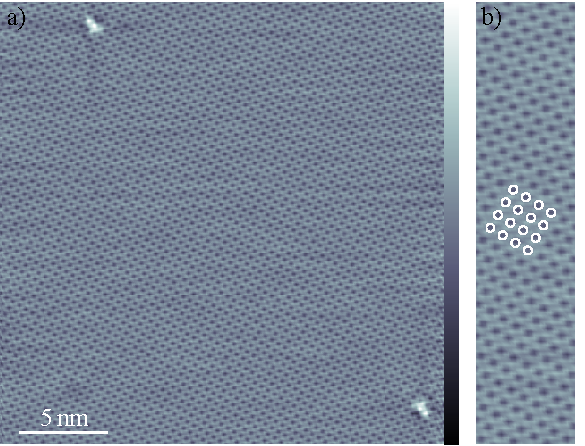
\includegraphics[width=\textwidth]{Ch4_Pristine_PtSn4.pdf}
	\caption{ }
	\label{fig:ch4_pristinetopo}
\end{figure}

\par In total, we took over 20000 STM topographies in this study, covering an area of over two million nanometer squared. More specifically, we acquired around 10000 images on 5 macroscopic spots on the HR$_1$ surface, around 5000 images on the HR$_2$ surface, and around 2000 images on 2 macroscopic spots on the LR$_1$ surface. 
Panel a) of \ref{fig:ch4_pristinetopo} exhibits a typical STM topography on PtSn$_4$, it is featured by waffle-like square corrugations and sparse defects at different atomic sites. Pristine cleaved surfaces are remarkably defect free, which we quantify through a careful statistical analysis in a subsequent section. We can overlay the Pt-layer to the surface of the pristine surface as shown in b) of \ref{fig:ch4_pristinetopo} and it maps perfectly with the square corrugations we observed. It might be tempting to say that we are typically scanning on the Pt-surface, but note that as mentioned in Ch.2, the tunneling current of STM has both the contribution of distance and electronic structure of the sample, the pattern revealed on topography is not necessarily the top most surface. To determine on what termination we are scanning, we ran a full terrace characterization.

\begin{figure}
	\centering
	\includegraphics[width=0.5\textwidth]{example-image-a} % Replace with your image file
	\caption{Placeholder for cleaving planes of PtSn$_4$}
	\label{fig:ch4_cleavingplane}
\end{figure}


\subsection{Terrace determination}
%todo: to insert the pdf showing potential cleaving planes of PtSn4.
\par Surface of PtSn$_4$ reveals flat terraces that belongs to different cleavage planes. Inspecting the crystal structure of PtSn$_4$, we note that there are three possible cleavage planes as shown in Fig 2. They are Sn$_a$-Pt, Pt-Sn$_b$, and Sn$_b$-Sn$_a$. Sn$_b$-Sn$_a$ bond has twice the length as Sn$_a$-Pt and Pt-Sn$_b$ bond and thus is weaker. We expect this material to cleave predominately between Sn$_b$-Sn$_a$. 

\begin{figure}
	\centering
	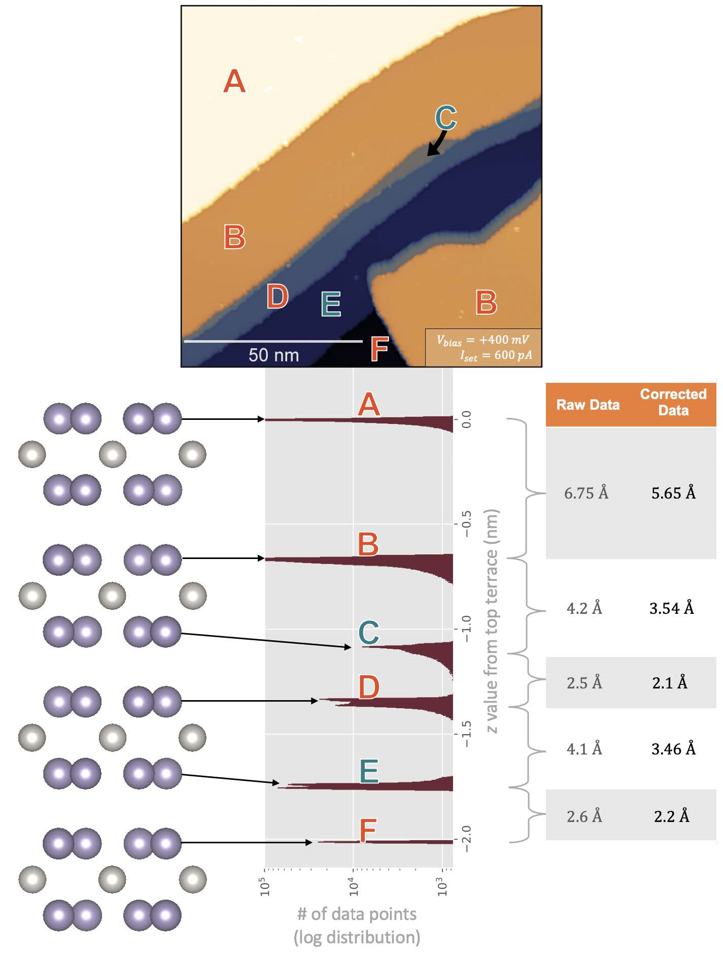
\includegraphics[width=\textwidth]{Ch4_termination.png}
	\caption{termination characterization}
	\label{fig:ch4_termination}
\end{figure}

\par In the experiment, we often landed our tips on a dominating terrace that is big and flat, and by scanning the step edges of the terraces, we could also see other terminations but with much less occurrence. To determine the dominating terrace we are scanning, we analyzed the step heights on a step-edge area, as shown in \ref{fig:ch4_termination}. 

Before we discuss the result shown in panel b) of \ref{fig:ch4_termination}, we need to understand how cleaving modifies the sample structure. Note that cleaving breaks the translational symmetry for the top layers; this effect is most profound for the surface layer where the covering layers are replaced by vacuum; the absence of support from the covering layers results in the surface layer to 'relax' into the surface, making the physical distance between the top most layer and the subsequent layer smaller than that of the normal lattice. However, how strong the relaxation effect is varies for different cleavage planes with different local bonding environments. There are two possible Sn-terminations in PtSn$_4$, and it is clear that compared to the relaxation of the Sn$_a$ termination due to Sn$_b$-Sn$_a$ cleaving, a Pt-Sn$_b$ cleaving will lead to a larger relaxation for the Sn$_b$ termination, as illustrated in \ref{fig:ch4_relaxation}. As a consequence, the relaxed height difference between Sn$_a$-Sn$_b$ terminations will be larger than 2.8 {\AA} (1/4 unit cell along the $b$-axis), and that of Sn$_b$-Sn$_a$ will be smaller than 2.8 {\AA}. That is precisely what we see in the height profile of step edge areas in panel b) of \ref{fig:ch4_termination}. Here, a height histogram is mapped from the topography and peaks can be assigned to different terminations. This analysis confirmed that the Sn$_a$ is the dominant termination we are scanning. Other terminations corresponding to the Pt and Sn$_b$ layer were seldom observed, accounting for less than 1\% of the total area investigated. 

\par For more details of the termination determination of PtSn$_4$, the reader can consult chapter 3 of Ashley Warner's thesis \cite{warner_defect_nodate}.

\begin{figure}
	\centering
	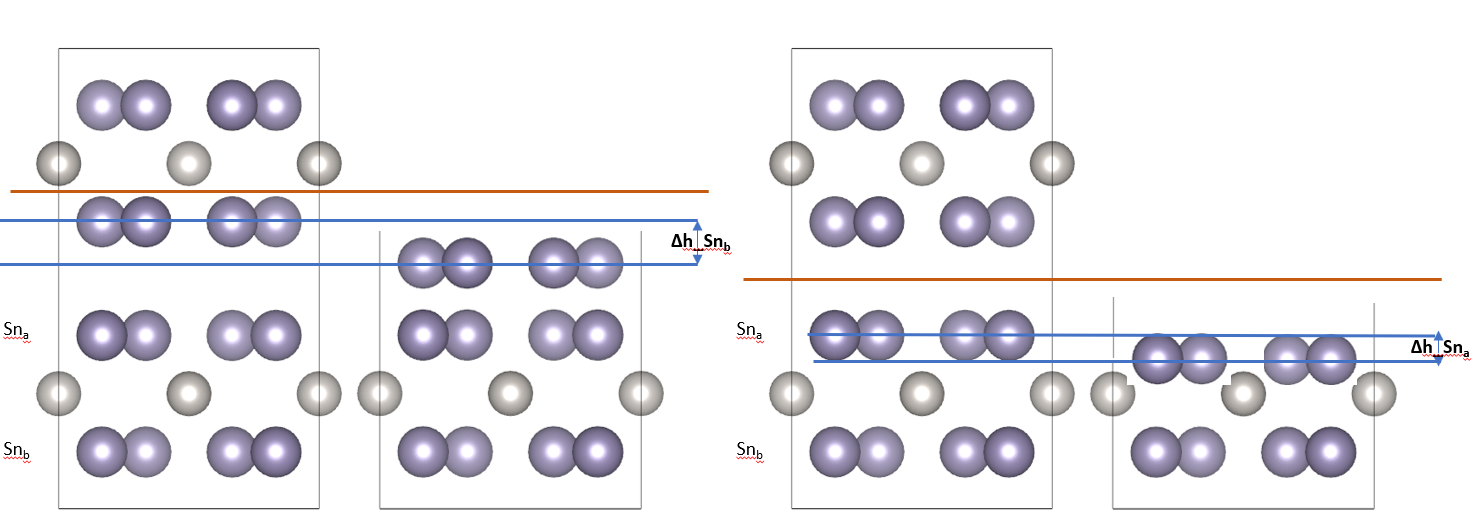
\includegraphics[width=\textwidth]{Ch4_relaxation.png}
	\caption{Relaxation}
	\label{fig:ch4_relaxation}
\end{figure}



\section{Defect Analysis}

\subsection{Defects in STM}
what is a defect?
Phenomenologically, defects are any disruptions in ideal, periodic lattice arrangement in STM topography. They can have different origins; for point defects, they can be due to site vacancy, substitution, adatoms on the surface, or interstitials that reside between layers.
Lattice imperfection breaks the local translational symmetry and is one the major sources of electron scattering in a metallic system. As the electron-phonon scattering and electron-electron scattering got supressed in low temperature, the temperature independent electron-defect scattering term dominates the residual resistance. Therefore, characterizing the defects in PtSn4 is crucial to understand the low temperature limit of resistance. In real space, electron-defect scattering process results in the outgoing electron being scattered with a modulated momentum and will thus create interference patterns around the scattering center, this modulation can be directly observed with STM spectroscopy, as the signal of differential conductance is proportional to the local density of state (LDoS) of electron. 
However, not all defects observed in STM can be considered a scattering center for the bulk material, as some defects can only reside on the surface or can be an artifact introduced by STM experiments.  For example, the adatoms defects are purely surface, with the cause being surface contamination either from the vacuum environment or from the tip, the adatom will never be observed in the bulk. 
In this study, we first identify different types of defects via topographic images, then we take point spectroscopy measurement on the defects ,and grid maps around defect rich areas to characterize their scattering behavior. In this section, we will present all the point defects types we observed in PtSn$_4$ and the their density via rigorous statistical analysis. 

\begin{figure}
	\centering
	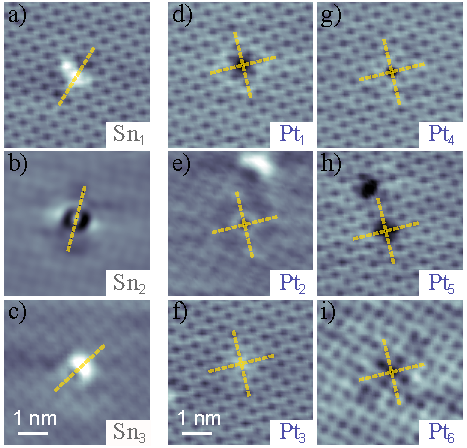
\includegraphics[width=\textwidth]{Ch4_defect_gallery.pdf}
	\caption{defect gallery}
	\label{fig:ch4_defectgallery}
\end{figure}

\subsection{Defects Topography}
Throughout the exploration on both fast-cooled and slow-cooled sample, different types of defects are observed, with the dominating source being point defects. In total, we observed 9 types of point defects in PtSn$_4$ as shown in \ref{fig:ch4_defectgallery}. 6 types are characterized as reside on Pt-sites and 3 on the Sn-site. Whether the defect belongs to a Sn-site or a Pt-site is determined with the lattice symmetry preserved in the Pt-layer and Sn-layer. As shown in \ref{fig:ch4_symmetry}, point defects sitting at the Pt-site will break the local translational symmetry, it changes the local electronic environment of 4 neighboring Pt atoms and thus exhibits a 2 fold symmetry and mirror symmetry in 2 axes(C$_2v$). As for Sn-layers, a modification on the Sn-site will result in a pattern with lower symmetry, with mirror symmetry in only 1 axis. Therefore, we can determine the origin of the defect based on the symmetry exhibited by the defect topography. 

\begin{figure}
	\centering
	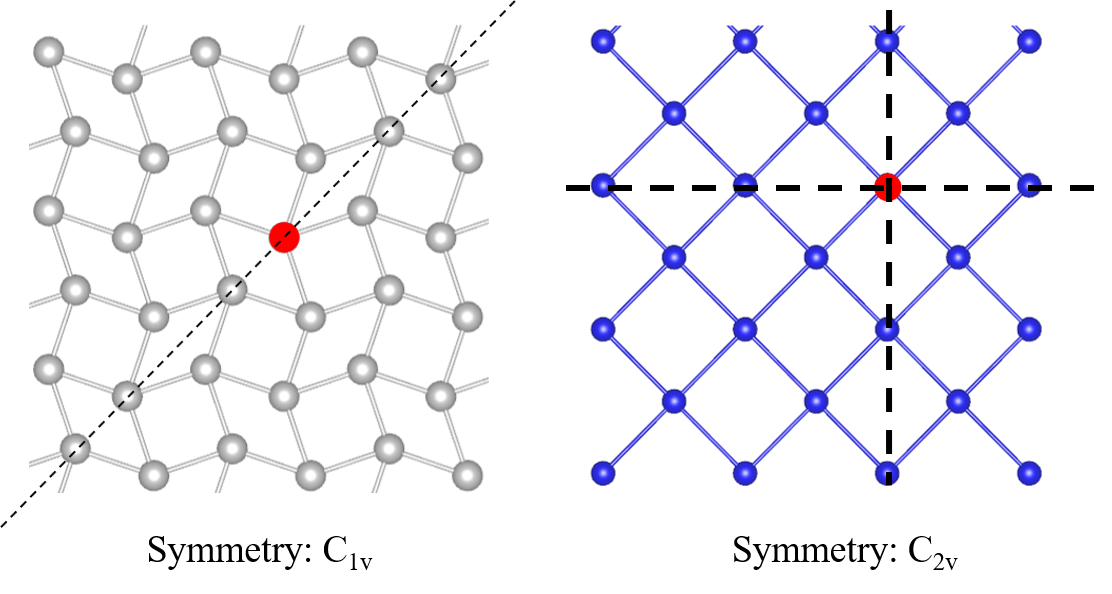
\includegraphics[width=\textwidth]{Ch4_symmetry.png}
	\caption{In plane lattice symmetry, left: Sn layer, right: Pt layer}
	\label{fig:ch4_symmetry}
\end{figure}

\subsection{Defect Statistics}

\subsubsection{Statistical Framework}
Defect density is a direct metric to evaluate the level of lattice perfection of a system. To achieve a reliable defect density and their associated undertainties, we used a statistical framework grounded in binomial and Poisson distribution principles, and justify its applicability to our experimental observations.
\par Our analysis of defect densities in PtSn4 crystals commences with the consensus that that point defects emerge as a stochastic process\cite{rudolph_defect_2010},\cite{mosquera-lois_imperfections_2023}. Given the crystal lattice structure, defects can randomly occur at any site, rendering each occurrence an independent event. This randomness and independence are fundamental assumptions that underpin our methodological approach, it is justified by STM topography as mentioned in the later paragraph.  
\par In total, 3 types of Sn-site defects and 6 kinds of Pt defects are observed. Since each site can only be occupied by one defect, to individual types of defect, we can conceptualize each lattice site as a discrete trial within a binomial framework. A 'success' in this context was defined as the presence of this particular type of point defect at a given site, denoted by '1', while its absence was considered a 'reference event', denoted by '0'. This binary scheme facilitated the application of the binomial distribution to model the statistics of defect occurrences across the lattice.
\par Given the expansive scanning area corresponding to a vast number of lattice sites (trial), coupled with the markedly low probability of defect occurrence (success rate), our analysis necessitated an approximation to simplify computations and enhance analytical tractability. The 
binomial distribution converges to the Poisson distribution under these conditions of large trial numbers and a small success rate. This approximation is underpinned by established statistical criteria. When the number of trials (n) exceeds 100 and the success rate (p) is below 0.1, the Poisson distribution serves as an effective surrogate for the binomial distribution. 
\par In our specific case, with n on the order of $10^5$ and p ranging between $10^-3$ and $10^-5$, the mean of the Poisson distribution ($\lambda=n\cdot p$) falls between 1 and 100. These are the conditions where the Poisson approximation is not only justified but advantageous, facilitating a more streamlined analysis of defect densities.
\par The sparse and non-clustered distribution of defects, as revealed through Scanning Tunneling Microscopy (STM) topographies, provided empirical validation for our methodological choices. The lack of defect clustering corroborates the assumption of defect occurrences as independent events, likely driven by thermal activation rather than mechanical strain. Mechanical strain would predictably induce clustering or patterned distributions of defects due to stress relaxation dynamics within the crystal lattice.
\par The transition from a binomial to a Poisson framework is further justified by the nature of our observations and the computational efficacy it offers. The Poisson distribution, known for its applicability to rare events in large populations, aligns well with the characteristics of defect formation in PtSn4 crystals. This alignment not only simplifies the mathematical treatment of defect statistics but also enhances the interpretability of our findings.

\subsubsection{Defect counting}
Defect counting is one of the key components to this study. Before the labour work of manually counting the defects, it is important to sample our image pool to avoid bias and enhance statistical representativeness. There are a few principles I followed with image selection: 
\begin{itemize}
	\item 1. Use images with good and consistent tip conditions(here the standard is whether the tip can image atomic resolution), but images taken at different bias voltages are allowed. 
	\par Rationale: Defects images taken by consistent tip conditions will give a more consistent pattern and thus more robust counting.	
	\item 2. Avoid repetitive areas. 
	\par Rationale: Many of the images are take on the same area to gauge the tip conditions.
	\item 3. Choose big size images, here we use images of size bigger than 50nm by 50nm.
	\par Rationale: Smaller size images are usually taken to focus on object of interest, thus biased.  
\end{itemize}  
Just to give the reader a sense, we collected around 20000 topographic images in our study, after standard 1, we are left with around 3000 images, then we apply standard 2, we again eliminate about 80\% of the images, and with standard 3, we are left with in total 55 images, with 33 on HR sample and 22 on LR samples. However, with the statistical framework we established in last section, the areas covered by these images are still big enough for us to make statistically meaningful claim on defect density.

\subsubsection{Defect density}

\begin{table*}
		\renewcommand{\arraystretch}{1.5}  % Increased line separation
		\caption{Defect statistics of two samples of PtSn$_4$ grown at two different cooling rates: slow-cooled sample S1 (RRR~$>1000$) and fast-cooled sample S2 (RRR~$=200$).} \label{tab:table1}
		\begin{tabular}{ccccc}
			Defect & Symmetry & Category & $\rho A_{\text{S1}}$ (per unit cell) & $\rho A_{\text{S2}}$ (per unit cell) \\ 
			\hline
			Sn$_1$ (Croissant)\footnote{This kind of defect is believed to be non-intrinsic} & $C_{1v}$ & Sn site & $1.00(0.02) \times 10^{-3}$ & $3.50(0.03) \times 10^{-3}$ \\
			Sn$_2$ (Spearhead)$^{\text{a}}$ & $C_{1v}$ & Sn site & $1.46(0.02) \times 10^{-3}$ & $0.216(0.008) \times 10^{-3}$ \\
			Sn$_3$ (Crescent)$^{\text{a}}$ & C$_{1v}$ & Sn site & $1.545(0.007) \times 10^{-4}$ & $0.033(0.009) \times 10^{-4}$ \\
			\hline
			Pt$_1$ & $C_{2v}$ & Pt site & $2.9(0.5) \times 10^{-5}$ & $5.6(0.4) \times 10^{-5}$ \\
			Pt$_2$ & $C_{2v}$ & Pt site & $3.8(0.5) \times 10^{-5}$ & $5.4(0.4) \times 10^{-5}$ \\
			Pt$_3$ & $C_{2v}$ & Pt site & $1.7(0.3) \times 10^{-5}$ & $2.1(0.3) \times 10^{-5}$ \\
			Pt$_4$ & $C_{2v}$ & Pt site & $2.8(0.4) \times 10^{-5}$ & Not Observed \\
			Pt$_5$ & $C_{2v}$ & Pt site & Not Observed & $2.0(0.2) \times 10^{-5}$ \\
			Pt$_6$ & $C_{2v}$ & Pt site & Not Observed & $0.5(0.1) \times 10^{-5}$ \\
			\hline
			Sn$_{\text{total}}$ &  &  & $2.61(0.03) \times 10^{-3}$ & $3.72(0.03) \times 10^{-3}$ \\
			Pt$_1$+Pt$_2$+Pt$_3$ &  &  & $0.84(0.08) \times 10^{-4}$ & $1.31(0.06) \times 10^{-4}$ \\
			Pt$_{\text{total}}$ &  &  & $1.1(0.08) \times 10^{-4}$ & $1.56(0.07) \times 10^{-4}$ \\
		\end{tabular}
\end{table*}

\par Defect densities for each type are reported in Table~\ref{tab:table1}. defect densities are reported on both the highRRR and lowRRR sample. Pt site defects are significantly rarer than Sn site defects, as discussed below. Of the 6 types of Pt-site defects, Pt$_{1}$,Pt$_{2}$ and Pt$_{3}$ were observed in both samples. All Pt site defects are in the range of 10--50 ppm, and of the three types present in both high and lower RRR samples, all increase in the fast-cooled lower RRR sample. The overall density of Pt site defects increases for the lower RRR sample, consistent with expectations from the increased low-temperature resistivity originating from point defect scatterers.

\par Defects residing on the Sn site are more prevalent in both samples, having densities that are between one and two orders of magnitude larger than the Pt site defects. However, the analysis is confounded by sensitivity to surface effects. Although significant increases in defects over time due to the adsorption of contaminants were not observed, other extrinsic variability appears to significantly influence the total Sn site defect density. In particular, the Sn$_1$ (croissant) defect is readily induced by the tip through voltage pulses or prolonged high voltage, and these defects have been observed to move and even annihilate, leading us to suspect these defects correspond to a Frenkel pair (a Sn adatom-Sn vacancy pair). The Sn$_2$ and Sn$_3$ defects anomalously decrease in the fast-cooled (lower RRR) sample, contrary to expectations from the transport measurements. We suspect these correspond to vacancies and/or adatoms that arise during cleaving, as the Sn surface is easily disturbed. With these extrinsic factors in mind contributing to the total observed defect density, we can only place an upper limit on the number of scattering sites. However, we note that as no new defect types appear, and all are sensitive to disorder reorganization of atoms, we do not observe any Sn-site defects corresponding to chemical substitutions - in other words, no other atoms are present on the Sn sites. While intrinsic Sn site defects are surely present, they are dominated by extrinsic ones, we will therefore focus more on the Pt site defects.

\par Having established that the Pt site defects provide a more reliable indicator of the intrinsic defect concentration, we can next examine the differences between samples S1 (higher RRR) and S2 (lower RRR). Pt$_1$, as the dominant intrinsic defect, doubled in the lower RRR sample, and the Pt$_2$ defect also has a sizable increase in the low RRR sample. And Pt$_3$ does not have a notable change in the density. Taken in aggregate the increase in defects corresponds to a $1.5\times$ larger concentration of Pt site defects in S2 with a lower RRR as compared to S1 with a higher RRR.  The increase in intrinsic defect densities is aligned with the decrease in the low-temperature resistivity across the two samples. However, naively, we would expect a linear correlation between defect concentration and residual resistivity due to electron-defect scattering. The observed increase of $1.5\times$ in the Pt site defects described here fails to account for the $5\times$ decrease in the RRR value for S2 as compared to S1. We therefore conclude that, although the Sn site defects are dramatically obscured by the non-intrinsic effects described above, they must account for the majority of increased scattering centers. 

\subsection{Non-Intrinsic Defects in PtSn$_4$} \textcolor{red}{In Appendix?}

\begin{figure}
	\centering
	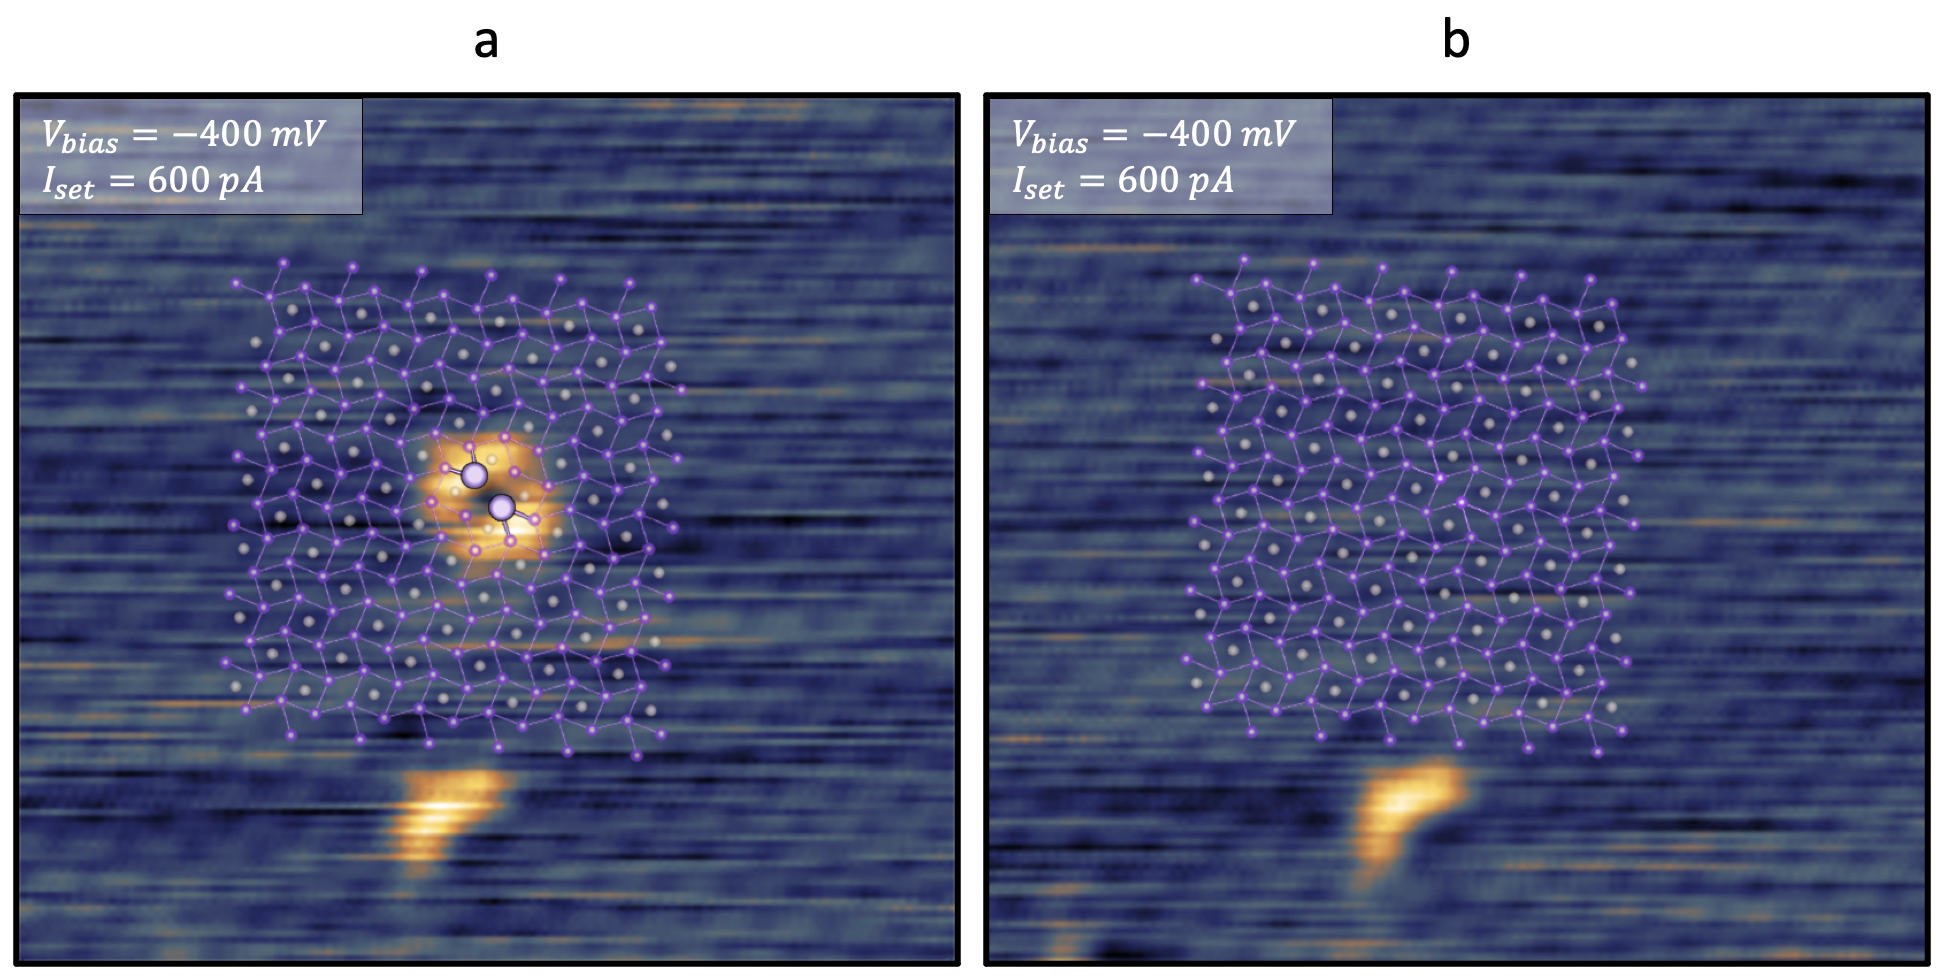
\includegraphics[width=0.8\textwidth]{Ch4_croissant.png}
	\caption{Two Sn$_1$ defect annihilation, indicating the origin of Sn$_1$ defects being from Frankel pairs}
	\label{fig:Ch4_croissantannihilation}
\end{figure}

\begin{figure}
	\centering
	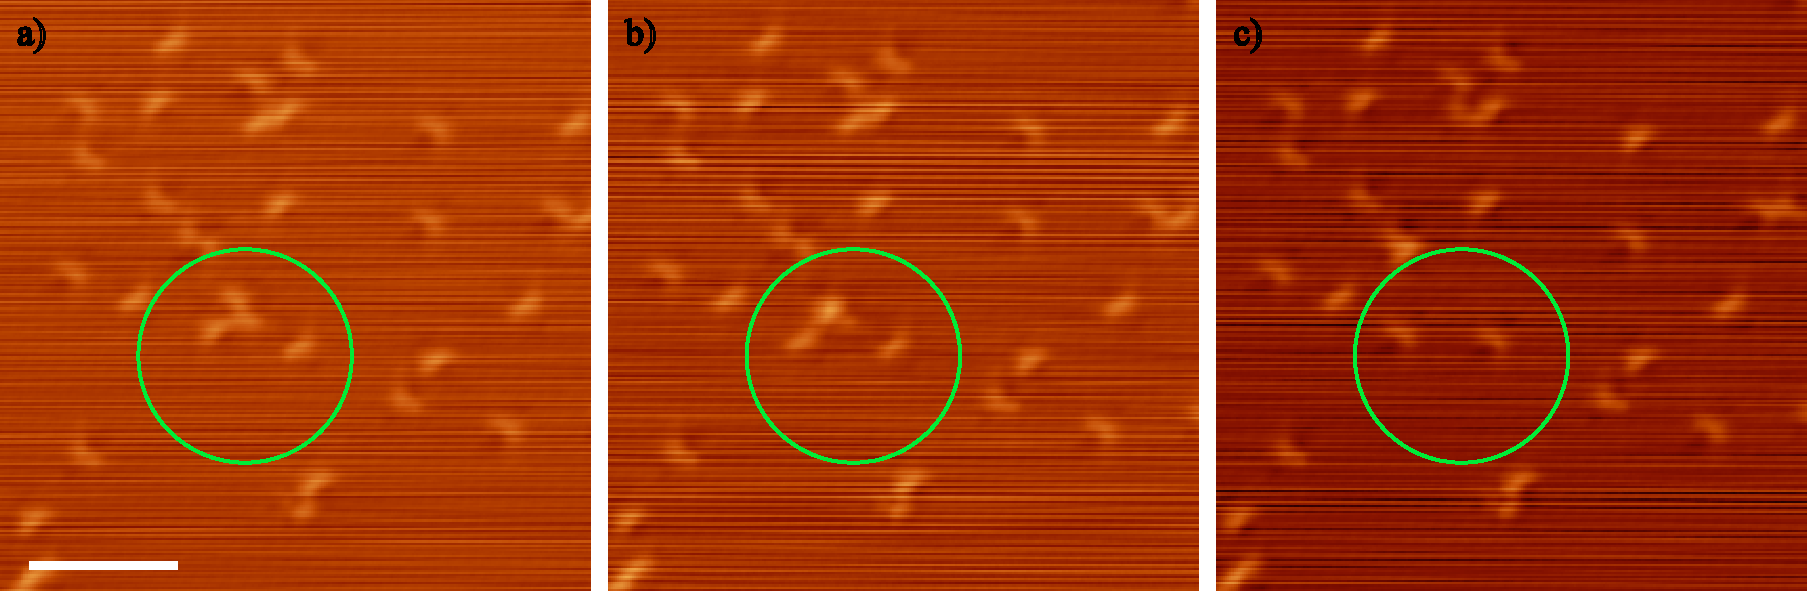
\includegraphics[width=0.8\textwidth]{Ch4_rotationcroissant.pdf}
	\caption{Sn$_1$ defect under consecutive scans, rotations and annihilation were found in the green circle.}
	\label{fig:Ch4_rotationcroissant}
\end{figure}

\par In our experiment, we have observed that the Sn1 defect, located at the Sn-site, is highly mobile under conditions of high scanning biases (exceeding 600mV). Notably, rotation of this defect is consistently observed in consecutive scans, example given in \ref{fig:Ch4_rotationcroissant}, and instances of annihilation between two Sn1 defects have also been documented, as shown in \ref{fig:Ch4_croissantannihilation} and \ref{fig:Ch4_rotationcroissant} b) to c). These events demonstrate the ability to both create and annihilate defects during scanning. This behavior also suggests that the origin of the Sn1 defect could be a Frankel pair on the Sn site. %could elaborate more on the origin of Sn1 defect. 
%todo: prepare figure on the population over different macroscopic spots. 
\par Moreover, the density of Sn1 defects varies significantly across different macroscopic locations on the crystal, as evidenced in STM observations (e.g., figure X). This variation, with density differences exceeding fiftyfold among explored locations, suggests that different cleaving planes may influence the introduction of Sn1 defects. Such spatial dependence supports the hypothesis that Sn1 defects could also be introduced during the cleaving process, reinforcing their classification as non-intrinsic.

\par While there is no direct evidence to suggest that Sn2 and Sn3 defects are non-intrinsic, the observed decrease in their densities from samples with higher residual resistivity ratio (RRR) to those with lower RRR supports the likelihood of these defects also being non-intrinsic. This variation could be indicative of differences in crystal order influenced by experimental conditions rather than intrinsic material properties.

\par In conclusion, while the intrinsic qualities of PtSn$_4$ are well-represented in STM studies, the influence of experimental techniques such as cleaving and scanning under bias voltage introduces a variety of non-intrinsic defects. However, it is worth noting that despite the ability to introduce these defects via experimental manipulations, these defects can still intrinsically exist in bulk samples, making the studies around these defects relevant. 

\section{discussion}
%todo: to write this section after ch.3 is finished
\par This section need to be written after the intro for PtSn4. ie Ch.2. 

\par This reasoning is consistent with both the numerically larger concentration of Sn atoms relative to Pt and the significantly reduced cost to form a Sn site vacancy as compared to a Pt Site vacancy as determined by DFT. Nonetheless, the dramatically small number of Pt site defects, where the occurrence of intrinsic defect is as rare as 1 in 10,000 unit cells, is good evidence that crystalline perfection is the underlying cause for the long mean free paths and hence the high RRRs observed in PtSn$_4$. 